\section{Zielsetzung}
\label{sec:Zielsetzung}

Das Ziel dieses Versuches ist die Untersuchung der Dipolrelaxation eines
strontiumdotierten Ionenkristalls aus Kaliumbromid.
Dafür wird die Relaxationszeit $\tau(T)$ der Dipole in den 
Kristallen bestimmt. Die Temperatur $T$ wird während des Versuches gemessen,
wogegen die Aktivierungsenergie $W$ und die charakteristische Relaxationszeit $\tau_{0}$
über den ebenfalls gemessenen Depolarisationsstrom berechnet werden können.

\section{Theorie}
\label{sec:Theorie}

Die Dipolrelaxation wird in diesem Versuch an Ionenkristallen beobachtet.
Werden die Dipole der Kristalle durch ein äußeres elektrisches Feld aus ihrer 
Gleichgewichtslage ausgelenkt, benötigen sie eine Zeit um sich nach Abschalten des 
elektrischen Feldes wieder in ihre Ausgangslage zurück zu bewegen. Der Übergang 
vom ausgelenkten Zustand zurück in den Ruhezustand wird als Relaxationsprozess 
bezeichnet. Die Dauer dieses Prozesses wird Relaxationszeit genannt.

\subsection{Dipole in Ionenkristallen}
\label{sec:Ionenkristalle}

Dieser Versuch wird an dem  Ionenkristall Kaliumbromid durchgeführt.
Ein Ionenkristall ist durch seine Eigenschaft definiert, abwechselnd aus Anionen
und Kationen aufgebaut zu sein.
Kaliumbromid besitzt eine einfach kubische Kristallstruktur,
da die Kaliumkationen (\ce{K}: $4s^1$ $\to$ \ce{K+}: $3p^6$) und die Bromanionen 
(\ce{Br}: $4p^5$ $\to$ \ce{Br-}: $4p^6$)
jeweils eine flächenzentriert kubische Struktur besitzen, die 
um eine halbe Gitterkonstante in eine Raumrichtung gegeneinander verschoben sind.
Dadurch ist das Kriterium der abwechselnden Kationen-Anionen-Anordnung 
erfüllt. Ein entsprechender Ionenkristall ist durch diese regelmäßige Ionenanordnung nach außen
elektrisch neutral. 
\begin{figure}
    \centering
    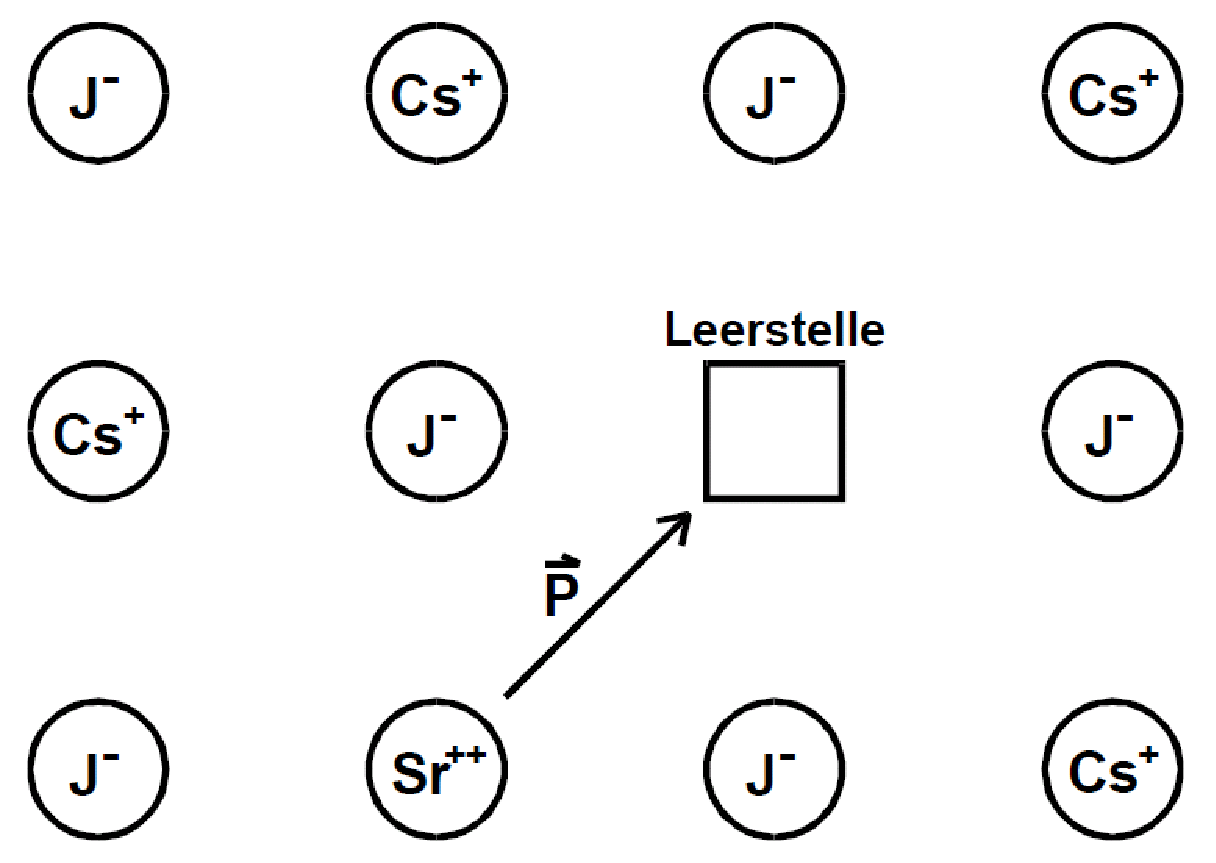
\includegraphics[width=0.6\textwidth]{figure/Dipol.pdf}
    \caption{Auf dieser Abbildung ist die Leerstellendiffusion aufgrund der 
    Dotierung von Cäsiumiodid mit Strontiumiodid dargestellt. Analoges gilt für 
    Kaliumbromid, wenn es mit Strontiumiodid dotiert wurde, da ebenfalls abwechselnd
    einfach geladene Kationen und Anionen die undotierte Gitterstruktur bilden. Der Vektor 
    $\vec{P}$ zeigt dabei die Ausrichtung der Dipole an, die durch eine Leerstelle und
    ein Strontiumion entstehen. \cite{2015}}
    \label{abb}
\end{figure}
Um die Enstehung von Dipolen im Kristall zu ermöglichen, wird 
die Probe mit einem Anteil von 0,005\% mit 
Strontiumiodid (\ce{Sr++}: $4p^6$ , \ce{I-}: $5p^6$) dotiert. Da Strontiumiodid zweifach positiv 
geladene Strontiumionen enthält, entstehen Kaliumleerstellen, die mit der 
zusätzlichen positiven Ladung einen Dipol bilden, damit die Gesamtladungsneutralität des
Kristalls aufrechterhalten werden kann. Dieses Verhalten ist in Abbildung \ref{abb}
dargestellt.
\FloatBarrier

\subsection{Dipolpolarisation}
\label{sec:Dipolpolarisation}

Die Dipole, welche sich aus den Strontiumkationen und den Leerstellen ergeben, 
sind entsprechend ihrer Position im Gitter ausgerichtet. Da nur diskrete 
Gitterplätze möglich sind, ist auch die Richtungsverteilung der Dipole bei 
Raumtemperatur statistisch diskret verteilt. Eine Richtungsänderung der 
Dipole ist durch Leerstellendiffusion möglich, wenn eine materialspezifische, 
thermische Aktivierungsenergie $W$ überschritten wird.
Die Anzahl der Dipole deren Energie ausreichend zur Diffusion ist, ist durch die 
Boltzmann-Verteilung gegeben. Das heißt, wenn die spezifische Aktivierungsenergie 
überschritten wird  (Umgebungstemperatur muss ausreichend hoch sein), dann bewegen sich 
die Dipole zurück in ihre Ausgangslage. Die Relaxation beginnt. 
Je größer die Umgebungstemperatur, desto mehr Energie steht den Dipolen zur Verfügung 
und desto schneller relaxieren sie. Das heißt die Relaxationszeit 

\begin{equation}
    \tau(T) = \tau_0 \exp{\left(\frac{W}{k_\text{B}T}\right)}
    \label{eq1}
\end{equation}

wird mit steigender Temperatur kleiner. Die Bewegung der Ladungsträger während der 
Relaxation führt zu einem Strom innerhalb des Kristalls, welcher 
Depolarisationsstrom genannt wird. Dieser kann mit Strom durch
weitere bewegliche Ladungsträger (z.B. aufgrund von Störstellen) überlagert werden
(Untergrund). Die Stromkurve ist in der folgenden Abbildung dargestellt.
\begin{figure}
    \centering
    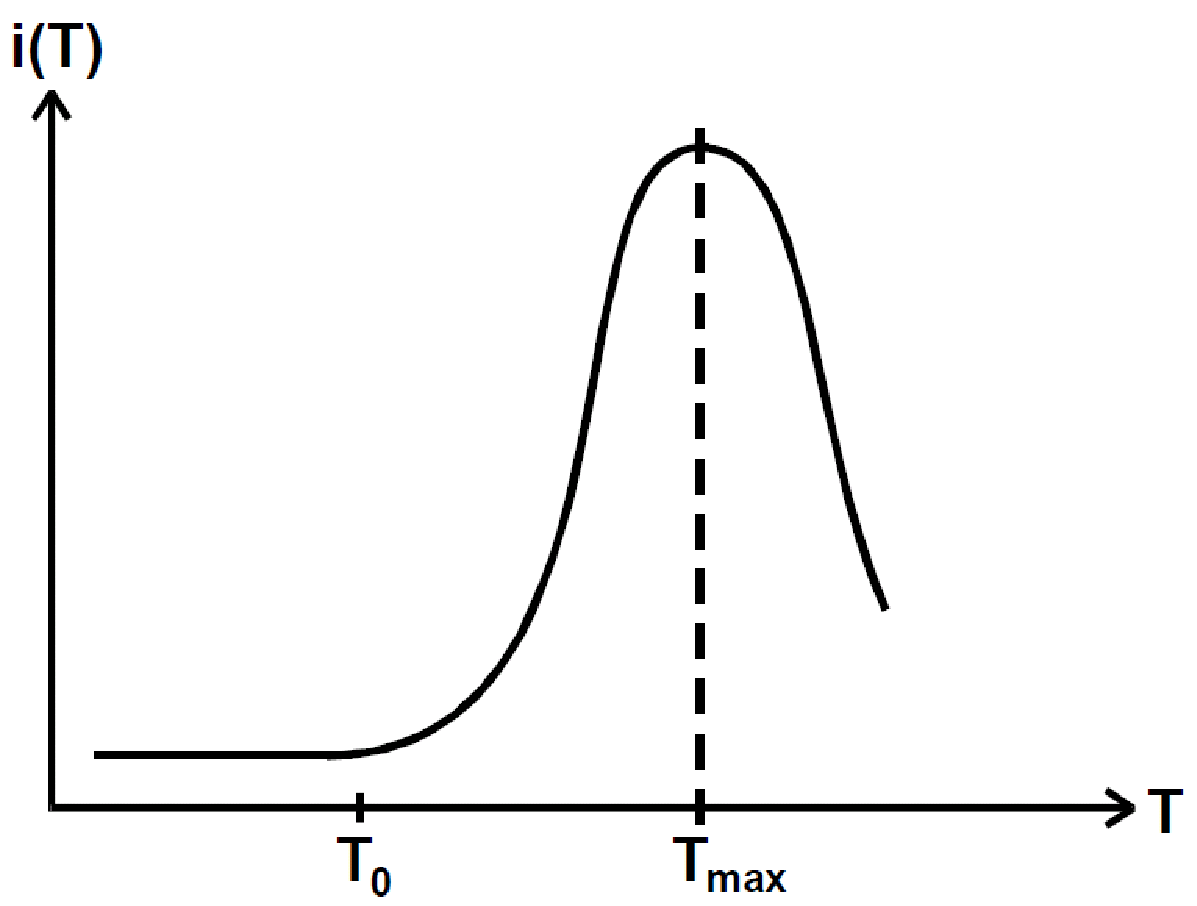
\includegraphics[width=0.6\textwidth]{figure/pol_strom.pdf}
    \caption{In dieser Graphik ist der Verlauf der Depolarisationsstromkurve
    abgebildet \cite{2015}.}
    \label{abb2}
\end{figure}
\FloatBarrier


\subsection{Berechnung der Aktivierungsenergie}
\label{sec:Aktivierungsenergie}

Um die Aktivierungsenergie zu bestimmen können zwei Ansätze verwendet werden,
wobei beide den Depolarisationsstrom beinhalten.
Der erste Ansatz wird über die Depolarisationsstromdichte
geführt. Dabei wird zunächst davon ausgegangen, dass diejenigen Dipole $y(T)$, die 
sich durch ein angelegtes elektrisches Feld ausgerichtet haben, durch 

\begin{equation*}
    y(T) = \frac{p E}{3 k_{\text{B}} T} 
\end{equation*}

gegeben sind. Der Depolarisationsstrom $j(t)$ kann dann mit den ausgerichteten 
Dipolen $y(T)$ über 

\begin{equation*}
    j(t) = y(T_{\mathrm{P}}) p \frac{\mathrm{d}N}{\mathrm{d}t}
\end{equation*}

ausgedrückt werden, wobei $p$ das Dipolmoment und 

\begin{equation*}
    \frac{\mathrm{d}N}{\mathrm{d}t} = -\frac{N}{\tau(T)}
\end{equation*}

die Stromdichte, also die pro Zeit und Volumeneinheit relaxierenden Dipole darstellt.
Eine Integration dieses Ausdrucks führt dann auf 

\begin{equation*}
    N = N_{\mathrm{P}} \exp{ \left( - \frac{ 1 }{ b } \int_{T_0}^T \frac{ \mathrm{d}T' }{ \tau(T') } \right )}
\end{equation*}

wobei $N_{\text{P}}$ die Anzahl der zu Beginn des Relaxationsprozesses
orientierten Dipole darstellt.
Die konstante Temperaturänderung ist definiert als

\begin{equation*}
    b = \frac{\symup{d}T}{\symup{d}t}.
\end{equation*}

Für den Depolarisationsstrom ergibt sich somit die Gleichung 

\begin{equation}
    j(T) = \frac{ p^{2} E }{ 3 k_{\mathrm{B}} T_{\mathrm{P}} } \frac{ N_{\mathrm{P}} }{ \tau_{\text{0}} } \exp{ \left( - \frac{ 1 }{ b \tau_{\text{0}} } \int_{T_{\text{0}}}^T \exp{ \left( - \frac{ W }{ k_{\mathrm{B}} T' } \right) \mathrm{d}T' } \right) } \exp{ \left( -\frac{ W }{ k_{\mathrm{B}} T } \right) } 
    \label{eq:j_T}
\end{equation}

wobei dieser Ausdruck für $T_{\text{0}} \approx T$ aufgrund des 
Zusammenhangs

\begin{equation*}
    \int_{T_{\text{0}}}^T \exp{ \left( - \frac{ W }{ k_{\mathrm{B}} T } \right )} \approx 0  
\end{equation*}

weiter zu 

\begin{equation}
    j(T) \approx \frac{ p^{2} E }{ 3 k_{\mathrm{B}} T_{\mathrm{P} }} \frac{ N_{\mathrm{P}} }{ \tau_{\text{0}} } \exp{ \left( - \frac{ W }{ k_{\mathrm{B}} T} \right ) }
    \label{eq2}
\end{equation}

approximiert werden kann.
Aus diesem Ergebnis kann schließlich die Aktivierungsenergie $W$ abgeleitet werden.
Eine weitere Möglichkeit zur Bestimmung von $W$ liegt in einem Ansatz, der über 
die Polarisation $P$ geführt wird.
Die zeitliche Ableitung der Polarisation ist als

\begin{equation*}
    \frac{\mathrm{d}P}{\mathrm{d}t} = - \frac{ P(t) }{ \tau(T(t))}
\end{equation*}

gegeben, wobei sie einen Strom $I(t)$ durch den Probenquerschnitt $F$ erzeugt und daher auch als

\begin{equation*}
    \frac{\mathrm{d}P}{\mathrm{d}t} = \frac{I(t)}{F} \qquad.
\end{equation*}

formuliert werden kann.
Somit lassen sich die oberen Gleichungen auf die Form 

\begin{equation*}
    \tau(T) = \frac{ \int_{T}^\infty j(T') \mathrm{d}T' }{ b j(T) } 
\end{equation*}

bringen. Wenn $\tau(T)$ durch Gleichung \eqref{eq1} ersetzt wird, kann 
die Aktivierungsenergie schließlich mit der Gleichung

\begin{equation}
    W = \ln{ \left( \frac{ \int_{T}^\infty j(T') \mathrm{d}T' }{ b j(T) \tau_{\text{0}} } \right) }k_{\mathrm{B}} T
    \label{eq3}
\end{equation}

bestimmt werden. In der Praxis gilt
$j(T \to \infty) = j(T^*)  \approx 0$.
Dieser Abschnitte wurde mittels des Literaturangaben 
\cite{Bucci}
\cite{Fuller}
\cite{Muccillo}
und
\cite{Becker}
erstellt.
\newpage